\documentclass{article}
\usepackage[T1]{fontenc}
\usepackage[lithuanian]{babel}
\usepackage{graphicx} % Required for inserting images
\usepackage{float} % For accuratelly placing images
\usepackage[a4paper, margin=2cm]{geometry}
\usepackage[hidelinks]{hyperref}
\usepackage{pdflscape}
\usepackage{longtable}
\usepackage{xltabular}
\usepackage{tabularx}
\usepackage{enumitem}

% For striketrghough
\usepackage{soul}

% For colored highlights 
\usepackage{xcolor}

% BEGIN: FOR SVG
% \usepackage[inkscapelatex=false]{svg}
\usepackage{svg}
\usepackage{amsmath}
% END: FOR SVG

\usepackage{everypage}
\usepackage{lscape} % Ensure landscape pages are recognized
\usepackage{lipsum}

\title{
    Įmonės „PTN“ procesų aprašymas \\
    \large versija 2.0 \\
    \large Komanda „PTN“}
\author{
    Greta Virpšaitė \\
    Rugilė Vasaitytė \\
    Domantas Keturakis \\
    Arnas Vaicekauskas \\
    \textbf{Liudas Kasperavičius (Lyderis)} 
}
\date{Spalis 2024}

\begin{document}
% \let\oldhl\hl
% \renewcommand{\hl}[1]{\oldhl{#1}}
\soulregister\workProdId7
\soulregister\processId7
\soulregister\prodWork7
\soulregister\process7
\soulregister\ref7
% Globals
\newcommand{\WorkProdIdsList}{}
\newcommand{\ProcIdsList}{}

\newcommand{\CheckUniqueWorkProd}[1]{
    \ifinlist{#1}{\WorkProdIdsList} {
    \PackageError{\WorkProdIdsList}{Work product "#1" already exists}{}
    } {
    \ifinlist{#1}{\ProcIdsList} {
        \PackageError{\ProcIdsList}{"#1" exists as a Process}{}
    } {
     \listgadd{\WorkProdIdsList}{#1}
    }
  }
}

\newcommand{\CheckUniqueProc}[1]{
    \ifinlist{#1}{\ProcIdsList} {
    \PackageError{\ProcIdsList}{Work product "#1" already exists}{}
    } {
    \ifinlist{#1}{\WorkProdIdsList} {
        \PackageError{\WorkProdIdsList}{"#1" exists as a Work product}{}
    } {
     \listgadd{\ProcIdsList}{#1}
    }
  }
}

% Work products
\newcommand{\WorkProdList}{}
\newcommand{\defineWorkProduct}[3]{%
  \expandafter\def\csname identifier#1\endcsname{#2}%
  \expandafter\def\csname name#1\endcsname{#3}%
  \CheckUniqueWorkProd{#2}
  \listgadd{\WorkProdList}{#1}
}
\newcommand{\workProdId}[1]{\textit{\csname identifier#1\endcsname}}
\newcommand{\workProdName}[1]{\csname name#1\endcsname}
\newcommand{\workProd}[1]{\workProdId{#1}. \workProdName{#1}}
\newcommand{\prodWork}[1]{\MakeLowercase{\workProdName{#1}} (\workProdId{#1})}

\newcommand{\describeWorkProd}[2]{
    \expandafter\def\csname desc#1\endcsname{#2}
}
\newcommand{\printRow}[1]{
        \workProdId{#1} &
        \workProdName{#1} &
        \csname desc#1\endcsname \\ \hline
}
\newcommand{\workProdDescriptions}{
    \forlistloop{\printRow}{\WorkProdList}
}

% Processes
\newcommand{\defineProcess}[3]{%
  \expandafter\def\csname procId#1\endcsname{#2}%
  \expandafter\def\csname procName#1\endcsname{#3}%
  \CheckUniqueProc{#2}
  \listgadd{\ProcList}{#1}
}
\newcommand{\processId}[1]{\textit{\csname procId#1\endcsname}}
\newcommand{\processName}[1]{\csname procName#1\endcsname}
\newcommand{\process}[1]{\processId{#1}. \processName{#1}}


\maketitle

\newpage
\tableofcontents

\newcommand{\WorkProdList}{}
\newcommand{\defineWorkProduct}[3]{%
  \expandafter\def\csname identifier#1\endcsname{#2}%
  \expandafter\def\csname name#1\endcsname{#3}%
  \listgadd{\WorkProdList}{#1}
}
\newcommand{\workProdId}[1]{\textit{\csname identifier#1\endcsname}}
\newcommand{\workProdName}[1]{\csname name#1\endcsname}
\newcommand{\workProd}[1]{\workProdId{#1}. \workProdName{#1}}
\newcommand{\prodWork}[1]{\MakeLowercase{\workProdName{#1}} (\workProdId{#1})}

\defineWorkProduct{ResourceEstimates}{ĮS}{Laiko, kainos ir žmogiškųjų išteklių sąmata}
\defineWorkProduct{FunReq}{FR}{Funkciniai reikalavimai}
\defineWorkProduct{NonFunReq}{NFR}{Nefunkciniai reikalavimai}
\defineWorkProduct{HighLevelArch}{ALSA}{Aukšto lygio sistemos architektūra}
\defineWorkProduct{Experience}{PP}{Įmonės patirtis su projektais}
\defineWorkProduct{ProjectScope}{PA}{Projekto apimtis}
\defineWorkProduct{Manual}{PNI}{Produkto naudojimo instrukcija}
\defineWorkProduct{Warranty}{GAS}{Garantinio aptarnavimo sutartis}
\defineWorkProduct{Ticket}{UK}{Užregistruota klaida}
\defineWorkProduct{UserNeeds}{VP}{Vartotojų poreikiai} % FIXME
\defineWorkProduct{Product}{PROD}{Produktas} % FIXME
\defineWorkProduct{Contract}{KS}{Sutartis su klientu} % FIXME
\defineWorkProduct{Backlog}{US}{Projekto užduočių sąrašas}
\defineWorkProduct{TechDocs}{TD}{Techninė dokumentacija} % FIXME

% SCRUM

\defineWorkProduct{SprintBacklog}{SUS}{Sprinto užduočių sąrašas}
\defineWorkProduct{SprintReviewDoc}{SPA}{Sprinto peržiūros ataskaita}
\defineWorkProduct{SotryPointRange}{PVI}{Pasakojimo vienetų intervalas}

\defineWorkProduct{ProductIncrement}{PP}{Produkto prieaugis}
\defineWorkProduct{Codebase}{PK}{Programinis kodas}
\defineWorkProduct{TechDoc}{TD}{Techninė dokumentacija}
\defineWorkProduct{DefectReport}{KL}{Klaidos}

\newcommand{\ProcList}{}
\newcommand{\defineProcess}[2]{%
  \expandafter\def\csname procId#1\endcsname{#1}%
  \expandafter\def\csname procName#1\endcsname{#2}%
  \listgadd{\ProcList}{#1}
}
\newcommand{\processId}[1]{\textit{\csname procId#1\endcsname}}
\newcommand{\processName}[1]{\csname procName#1\endcsname}
\newcommand{\process}[1]{\processId{#1}. \processName{#1}}

\defineProcess{EngageClient}{Kliento įtraukimas}
\defineProcess{DraftBacklog}{Užduočių sąrašo rengimas}

\defineProcess{CreateManual}{Naudojimo dokumentacija}
\defineProcess{CloseProject}{Projekto užbaigimas}
\defineProcess{BugFix}{Klaidos taisymas}

\section{Įmonės aprašymas}

\subsection{Įmonės pavadinimas}
"PTN"

% \subsection{"PTN" departments}

% \begin{enumerate}
%     \item  IT division
% \end{enumerate}

\subsection{Įmonės aprašymas}

% \textbf{NOTE:} Reikia aprašyti TIK IT depertamentą \newline

"PTN" yra projektinė įmonė. "Produktų vystymo" departamentas yra "PTN" IT departamentas, kuris užsiima e.komercijos sistemų kūrimu klientams. "Produktų vystymo" departamentas įdarbinę apie 30 darbuotojų. 

\subsection{Organizacinė struktūra}
Šiame dokumente mes modeliuojame tik IT departamentą pavadinimu "Produktų vystymo", kuris prisiima projektus susijusius su e.komercija.
\begin{table}[h!]
\centering
\begin{tabular}{p{0.1\textwidth}|p{0.9\textwidth}}
\hline
\textbf{Rolės} & \textbf{Atsakomybės} \\ \hline


% product developement & 

Projektų vadovas & \st{Manages and supervises the project, including setting project goals, timelines, and budgets. The project manager ensures that the development team meets deadlines and that the project is delivered successfully within the agreed-upon scope. They also act as the main point of communication between the client and the development team.}

Valdo ir prižiūri projektą, įskaitant projekto tikslų, terminų ir biudžetų nustatymą. Projekto vadovas užtikrina, kad programinės įrangos kūrimo (software development) komanda laikytųsi terminų ir kad projektas būtų sėkmingai įgyvendintas sutarta apimtimi. Jie taip pat tarpininkauja kliento ir programinės įrangos kūrimo (software development) komandos bendravime.

\\ \hline
% Deployment & Integrate developed systems with existing client platforms, for example: inventory or payment gateways. Maintain the internal IT infrastructure of the client companies. \\ \hline
Programinės įrangos kūrėjas (Software developers) & \st{ Responsible for developing the custom e-commerce software in line with the project's specifications. They ensure the functionality of the system through testing and work closely with the project manager to make sure client requirements are met. Developers also address all issues or bugs that arise during the development process. }

Atsakingas už pritaikytos e.komercijos programinės įrangos kūrimą pagal projekto specifikacijas. Testuotojai užtikrina sistemos funkcionalumą testuodami ir glaudžiai bendradarbiaudami su projekto vadovu, siekiant užtikrinti, kad būtų patenkinti kliento reikalavimai. Programinės įrangos kūrėjai (Software developers) taip pat sprendžia visas problemas ar sistemos klaidas, kurios kyla kūrimo proceso metu.
\\ \hline

Testuotojas & \st{Responsible for evaluating the functionality and quality of software. They conduct various types of testing to identify defects before the product is delivered and work closely with developers to validate fixes to their reported defects. }


Atsakingas už programinės įrangos funkcionalumo ir kokybės įvertinimą. Jie atlieka įvairių tipų testavimą, kad nustatytų defektus prieš pristatant produktą ir glaudžiai bendradarbiauja su programinės įrangos kūrėjais (Software developers), kad patvirtintų praneštų defektų pataisas.
\\ \hline

Architektas & \st{Designs the overall structure of the e-commerce software. The architect collaborates with developers to guide implementation and resolve complex technical challenges. }
Sukuria bendrą e.komercijos programinės įrangos struktūrą. Architektas bendradarbiauja su programininės
įrangos kūrėjais (software developers), siekdamas juos vesti įgyvendinimo procese ir padeda išspręsti sudėtingus techninius iššūkius.

\\ \hline
Analistas &  \st{Gather and analyse client requirements to ensure the project meets business needs.}

Surinka ir analizuoja klientų poreikius, kad įsitikintų, jog projektas atitinka verslo poreikius.
\\ \hline
% Projects & Manage and supervise project progress, develop project plans, and ensure the successful delivery of these systems within the agreed timelines and budgets. \\ \hline
% System Maintenance & Provide ongoing maintenance for live e-commerce platforms. Communicate with clients regarding system performance and to resolve any incidents or issues that arise. \\ \hline

% Paminėti, kad garantiniai atvejai

\end{tabular}
%\caption{Organizational Structure}
%\label{table:organizational_structure}
\end{table}


% \subsection{IT division}

% The IT department employs around 30 people. It carries out projects for private and public organisations and develops and maintains web applications in various fields.

% Short department description

% Project-based organisational structure

% E-commerce

% Agile/SCRUM

% Develops products and transfers them to the customer

% \subsubsection{Additional information}

% \paragraph{Organisational structure}
% \paragraph{Technologies used}
% \paragraph{Methodologies}




% svg debiliškai gaunas, sueis screeshot'as for the moment
% redaguoti galima čia https://demo.bpmn.io/s/start
% originalus failas: processes.bpmn

\begin{landscape}
\section{Procesų aprašymas}
\thispagestyle{empty}
\begin{figure}[H]%[htpb!]
    \centering
    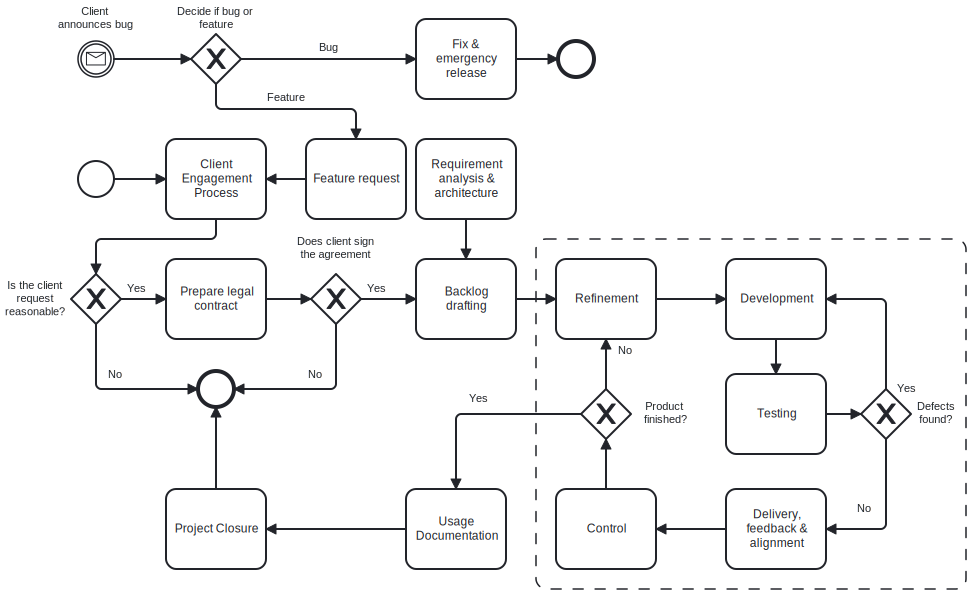
\includegraphics[width=\linewidth]{etc/diagram.png}
\end{figure}
\end{landscape}

\subsection{\process{EngageClient}} % ARNAS

\begin{figure}[H]%[htpb!]
    \centering
    \includegraphics[width=0.75\linewidth]{etc/engage-client.png}
\end{figure}

\begin{processTable}{EngageClient}
    \tikslas{Įvertinti kliento poreikius, rasti kompromisą dėl projekto sąmatos bei apimties ir pasirašyti sutartį}
    \inputs{
        \item \textit{KP}. Kliento poreikiai ir galimybės
        \item \workProd{Experience}
    }
    \outputs{   
        \item \workProd{ResourceEstimates}
        
        \item \workProd{ProjectScope}
        
        \item \workProd{Contract}
    }
    \veiklos{
         \item Projektų vadovas, architektas ir analitikas bendrauja su klientu, aiškinasi jo poreikius sistemai ir vertina kliento galimybes finansuoti tokios sistemos kūrimą. Ši veikla tęsiasi tol, kol įmonės atstovai surenka pakankamai informacijos paruošti klientui pasiūlymą.
    
        \item Projektų vadovas, architektas ir analitikas tarpusavyje įvertina kliento norus ir galimybes ir paruošia sutartį į kurią įeina laiko, kainos ir žmogiškųjų ištekliu sąmata bei nusakoma sistemos apimtis. \label{activity:prepare-deal}

        \item Klientui yra pateikiama sutartis. Jei klientas yra patenkintas sutarties sąlygomis pereinama prie sutarties pasirašymo \ref{activity:sign}. Klientas gali nesutikti su sutarties sąlygomis. Tokiu atveju klientas pateikia naujus poreikius ir dar kartą vykdoma veikla \ref{activity:prepare-deal}. Jei abi šalys nesugeba rasti kompromiso, procesas gali būti nutrauktas ir darbas su klientu netęsiamas.

        \item Pasirašoma sutartis su klientu. \label{activity:sign}
    }
\end{processTable}

\newpage
\subsection{\process{RA}} % DOMANTAS

\begin{processTable}{RA}
    \tikslas{Nustatomi reikalavimai, kuriuos turi atitikti sistema, atitinkamai suprojektuojama sistema.Surinkti/nustatyti/išvesti? funkcinius ir nefunkcinius reikalavimus}
    % Surinkti/nustatyti/išvesti? funkcinius ir nefunkcinius reikalavimus
    % Derive technical requirements that the system must meet and design the system accordingly.
    \inputs{
       \item \workProd{Kazkas}
    }
    \outputs{
       \item \workProd{Kazkas}
    }
    \veiklos{
        \item Kazkokia veikla
    }
\end{processTable}

\begin{table}[h!]
\begin{tabular}{p{0.1\textwidth}|p{0.8\textwidth}}
\hline
\textbf{\processId{RA}}    & \textbf{\processName{RA}} \\ \hline
Tikslas & 
Nustatomi reikalavimai, kuriuos turi atitikti sistema, atitinkamai suprojektuojama sistema.
Surinkti/nustatyti/išvesti? funkcinius ir nefunkcinius reikalavimus

Derive technical requirements that the system must meet and design the system accordingly. \\ \hline

Naudojami darbo produktai &
\begin{itemize}
    \item \workProd{ResourceEstimates}
    
    \item \workProd{ProjectScope}
\end{itemize}
\\ \hline
Sukurti darbo produktai &
\begin{itemize}
    \item \workProd{FunReq}
    \item \workProd{NonFunReq}
    \item \workProd{HighLevelArch}
    % Architecture
\end{itemize}
\\ \hline
Veiklos &   
\begin{enumerate}

    \item Identifikuojamos suinteresuotos šalys ir informacijos šaltiniai.
    \item Renkama informacija iš suinteresuotų šalių per interviu ir modeliuojami įmonės
    procesai iš identifikuotų informacijos šaltinių.
    \item Iš surinktos informacijos identifikuojami konkretūs vartotojų poreikiai
    % \item Perform analysis of gathered intel, document concrete user needs (\textit{UN}).
    \item Apibrėžiami funkciniai ir nefunkciniai reikalavimai iš identifikuotų vartotojų poreikių; laiko kainos, žmogiškųjų išteklių sąmatos ir projekto apimties.
    \item Aukšto lygio sistemos architektūra sukuria atsižvelgiant į apibrėžtus funkcinius ir nefunkcinius reikalavimus.
\end{enumerate}
\\ \hline
\end{tabular}

\label{pro/plan}
\end{table}

\newpage

\subsection{\process{DraftBacklog}} % ARNAS

\begin{table}[h!]
\begin{tabular}{p{0.1\textwidth}|p{0.85\textwidth}}

\hline

\textbf{\processId{DraftBacklog}} & \textbf{\processName{DraftBacklog}} \\ 

\hline

Tikslas &
Paversti analizės metu išgrynintus reikalavimus ir sistemos architektūra į panaudos atvejus ir technines užduotis iš kurių būtų sudaromas užduočių sąrašas. \\ 

\hline

Panaudoti darbo produktai & 

\begin{itemize}
    \item \workProd{FunReq}
    \item \workProd{NonFunReq}
    \item \workProd{HighLevelArch}
\end{itemize}

\\ \hline

Sukurti darbo produktai &

\begin{itemize}
    \item \workProd{Backlog}
\end{itemize} \\ 

\hline

Veiklos &

\begin{enumerate}
    \item Architektas kartu su analitiku agreguoja analizės metu surinktus reikalavimus bei aukšto lygio sistemos architektūra į panaudos atvejus ir atskiras technines užduotis. Kiekvienas panaudos atvejis ir techninė užduotis yra detaliai aprašomi
\end{enumerate} \\ 

\hline

\end{tabular}
\label{pro/back}
\end{table}

\newpage
\subsection{PRO/SCRUM. SCRUM CYCLE }

\subsubsection{PRO/REF. Refinement }

\begin{table}[h!]
\begin{tabular}{l|p{0.725\textwidth}}
\hline
\textbf{PRO/REF}        & \textbf{Refinement} \\ \hline
Purpose & Review and refine the backlog of tasks by breaking them into smaller, more manageable parts. Adjust priorities and ensure clarity in the tasks to align with the product goals and decide what and who will execute it this sprint. \\ \hline
Used work products (IN)   &      
\begin{itemize}
    \item \textit{PB}. Project backlog
    \item \textit{SP}. Story points range
    \item \textit{SRR}. Sprint review report
\end{itemize}
\\ \hline
Created work products (OUT) &     
\begin{itemize}
    \item \textit{PB}. Project backlog
    \item \textit{SB}. Sprint backlog
\end{itemize}
\\ \hline
Activities            &   
\begin{enumerate}
    \item The current \textit{PB} with the team is reviewed, focusing on any new \textit{PB} items added.
    \item Large tasks are broken into smaller, atomic tasks.
    \item Clarity in the task descriptions for better understanding and execution are ensured.
    \item The scrum team  estimates the effort required for each task using story points, typically following the Fibonacci sequence.
    \item Tasks based on current goals and resources are reassessed and prioritised, taking into the consideration \textit{SRR}.
    \item Selected tasks for the cycle with total work load fitting into the story points range (\textit{SP}) for the cycle, creating a sprint backlog (\textit{SB}).
    \item Team members plan who will execute each task.  
\end{enumerate}
\end{tabular}
\label{PRO/REF}
\end{table}

\newpage
\subsubsection{PRO/DEV. Development}

\begin{table}[h!]
\begin{tabular}{l|p{0.725\textwidth}}
\hline
\textbf{PRO/DEV}        & \textbf{Development} \\ \hline
Purpose & To implement the tasks listed in the sprint backlog according to the plan. The scrum team focuses on delivering potentially shippable product increments, ensuring the quality and functionality of the features. \\ \hline
Used work products (IN)    &      
\begin{itemize}
    \item \textit{SB}. Sprint backlog
    \item \textit{DR}. Defect report (conditional, if any defects are found int PRO/TEST)
    \item \textit{CODE}. Code-base
\end{itemize}
\\ \hline
Created work products (OUT) &     
\begin{itemize}
    \item \textit{PI}. Product increment 
    \item \textit{CODE}. Updated code-base.
    \item \textit{DOC}. Technical documentation 
\end{itemize}
\\ \hline
Activities            &   
\begin{enumerate}
    \item Each developer develops tasks as defined in the sprint backlog. Time spent on \textbf{2-7} activities must be logged in (\textit{SB}) for future alignment of tasks. 
    \item They write and maintain code following coding standards, updating the code-base (\textit{CODE}). 
    \item They write unit test with the line coverage of 70\% to ensure code quality and functionality, updating the code-base (\textit{CODE}).
    \item When code and unit tests are written, another team member must review the code. If any  changes are requested the processes is repeated from \textbf{2-4}.
    \item Once development is completed, all defects (\textit{DR}) have been addressed, and the code has been approved by another developer, the product increment (PI) for testing is prepared. The task status in the sprint backlog (SB) must be updated to reflect that the task is testable.
    \item Any necessary documentation (\textit{DOC}) must be written as well.
\end{enumerate}
\end{tabular}
\label{PRO/DEV}
\end{table}

\newpage
\subsubsection{PRO/TEST. Testing}

\begin{table}[h!]
\begin{tabular}{l|p{0.725\textwidth}}
\hline
\textbf{PRO/TEST}        & \textbf{Testing} \\ \hline
Purpose & To verify that the product increment meets the defined acceptance criteria and quality standards without breaking something in previous product increments. Testing ensures the product is functional, reliable. \\ \hline
Used work products (IN)    &      
\begin{itemize}
    \item \textit{PI}. Product increment
    \item \textit{DOC}. Technical documentation
    \item \textit{SB}. Sprint backlog
\end{itemize}
\\ \hline
Created work products (OUT) &     
\begin{itemize}
    \item \textit{DR}. Defect reports
    \item \textit{SB}. Updated sprint backlog
\end{itemize}
\\ \hline
Activities            &   
\begin{enumerate}
    \item Testers must log work done in \textbf{2-6} in sprint backlog (\textit{SB}).
    \item Testers review the product increment (\textit{PI}) against acceptance criteria (from \textit{SB}) and requirements, using \textit{DOC} if necessary.
    \item They perform functional and non-functional testing (e.g. integration, system, performance, and security testing) as per requirements of the tasks.
    \item They conduct regression testing (automated) to ensure new changes do not affect existing functionality.
    \item They update defect reports (\textit{DR}) to reflect the quality status.
    \item If defects are found, the task loops back into the development cycle to address the issues. The tester must change the status of the task to reflect that it is back in development in the sprint backlog (\textit{SB}).
\end{enumerate}
\end{tabular}
\label{quality_assurance_process}
\end{table}

\newpage
\subsubsection{PRO/PD. Partial delivery \& feedback}

\begin{table}[h!]
\begin{tabular}{l|p{0.725\textwidth}}
\hline
\textbf{PRO/PD}        & \textbf{Partial delivery \& feedback} \\ \hline
Purpose & To deliver a  product increment to stakeholders and gather feedback. This process ensures that the product is moving in the right direction and that stakeholder expectations are met. \\ \hline
Used work products (IN)    &      
\begin{itemize}
    \item \textit{PI}. Product increment
    \item \textit{DR}. Defect reports
    \item \textit{PB}. Project backlog
\end{itemize}
\\ \hline
Created work products (OUT) &     
\begin{itemize}
    \item \textit{FD}. Feedback documentation
\end{itemize}
\\ \hline
Activities            &   
\begin{enumerate}
    \item Deliver the product increment (\textit{PI}) to stakeholders for initial feedback.
    \item Present the outcomes of the latest sprint, including the features developed and known issues from \textit{DR}.
    \item Collect feedback from stakeholders regarding the delivered increment and its alignment with their needs. Discuss any gaps, potential improvements, and changes to the     \textit{PB}.
    \item Write feedback documentation (\textit{FD}).
\end{enumerate}
\end{tabular}
\label{partial_delivery_feedback_alignment}
\end{table}

\newpage
\subsubsection{PRO/CONTROL. Control (sprint review \& alignment)}

\begin{table}[h!]
\begin{tabular}{l|p{0.725\textwidth}}
\hline
\textbf{PRO/CONTROL}        & \textbf{Control (sprint review \& alignment)} \\ \hline
Purpose & To review and demonstrate the work completed during the sprint, allowing the team to self-evaluate how the sprint went. Feedback from stakeholders is also considered to assess time management and align on improvements for future scrum cycles. \\ \hline
Used work products (IN)    &      
\begin{itemize}
    \item \textit{PI}. Product increment
    \item \textit{DR}. Defect reports
    \item \textit{SB}. Sprint backlog
    \item \textit{EST}.  Resource, time and cost estimates
    \item \textit{SP}. Story point range
    \item \textit{FD}. Feedback documentation
    \item \textit{PB}. Project backlog
\end{itemize}
\\ \hline
Created work products (OUT) &     
\begin{itemize}
    \item \textit{SRR}. Sprint review report summarising the sprint's outcomes 
    \item \textit{SP}. Updated story point range 
\end{itemize}
\\ \hline
Activities            &   
\begin{enumerate}
    \item The team reflects on the sprint's progress, discussing what went well and what challenges were encountered.
    \item The project managed assesses the actual time spent on tasks compared to the initial estimates to understand the team's time management using sprint backlog (\textit{SB}) logged hours and initial time estimates (\textit{EST}).
    \item Based on \textbf{1-2} and feedback documentation (\textit{FD}), the project manager and scrum team identifies necessary adjustments for the next sprint. This includes updating the project backlog (\textit{PB}), reprioritizing tasks as needed and capturing these changes in the sprint review report (\textit{SRR}), refining the story point range (\textit{SP}).
    \item The project manager closes project if necessary - if no further sprints are required, they transition to usage documentation.
\end{enumerate}
\end{tabular}
\label{control_process}
\end{table}


\newpage
\subsection{\process{CreateManual}}

\begin{processTable}{CreateManual}
    \tikslas{Paruošti produkto naudojimo instrukciją, suprantamą naudotojams}
    \inputs{
        \item \workProd{UserNeeds}
        \item \workProd{UseCases}
        \item \workProd{Product}
    }
    \outputs{
            \item \workProd{Manual}
    }
    \veiklos{
         \item Detaliai aprašomi visi žingsniai kiekvienam panaudos atvejui (\workProdId{UseCases}) naudojant produktą (\workProdId{Product}). \label{CreateManual/1}
        \item Detaliai aprašomos visos produkto (\workProdId{Product}) funkcijos (t.y. kaip jomis pasinaudoti) \label{CreateManual/2}
        \item Iš \ref{CreateManual/1}. ir \ref{CreateManual/2}. sudaromas struktūrizuotas, vientisas dokumentas - \prodWork{Manual}
        \item Atliekama produkto naudojimo instrukcijos (\workProdId{Manual}) validacija - paruoštas dokumentas peržiūrimas kolegų iš kitų padalinių, įsitikinama, jog instrukcija suprantama pirmą kartą produktą (\workProdId{Product}) naudojantiems žmonėms \label{CreateManual/3}
        \item Kol netenkinamas \ref{CreateManual/3}. punktas, atliekami naudojimo instrukcijos pakeitimai
        }
\end{processTable}

\begin{figure}[h]
    \centering
    \includegraphics[width=0.75\linewidth]{etc/diagrams/Manual.png}
\end{figure}
% --------------------------------------------------------------------
\newpage
\subsection{\process{CloseProject}}
\begin{processTable}{CloseProject}
    \tikslas{Užbaigti projektą, perduoti paruoštą naudojimui produktą klientams}
    \inputs{
        \item \workProd{Product}
    	\item \workProd{Contract}
    	\item \workProd{Backlog}
    	\item \workProd{TechDocs}
    	\item \workProd{Manual}
    }
    \outputs{
        \item \workProd{Warranty}
        \item \workProd{Experience}
    }
    \veiklos{
         \item Įsitikinama, jog visos užduočių sąraše (\workProdId{Backlog}) numatytos užduotys yra įgyvendintos
        \item Atliekami sutartyje (\workProdId{Contract}) numatyti produkto (\workProdId{Contract}) perdavimo klientui darbai
        \item Klientui perduodama \prodWork{Manual}
        \item Klientui perduodama \prodWork{TechDocs}
        \item Sudaroma ir pasirašoma \prodWork{Warranty}, kurioje numatomas garantinio aptarnavimo laikotarpis
    	\item Atliekama vidinė komunikacija apie užbaigtą projektą. Projekto vadovas dalinasi projekto eiga, priimtais kritiniais sprendimais ir rezultatais. Taip kaupiama \prodWork{Experience} 
    	\item Kol nesibaigia sutartyje (\workProdId{Contract}) numatytas adaptacinis laikotarpis, klientams teikiama techninė pagalba
    }
\end{processTable}

\begin{figure}[!h]
    \centering
    \includegraphics[width=0.8\linewidth]{etc/diagrams/projectClosure.png}
\end{figure}
\newpage

%----------------------------------------


\subsection{\process{BugFix}}
\begin{processTable}{BugFix}
    \tikslas{Ištaisyti ne dėl kliento kaltės kilusias produkto klaidas}
    \inputs{
        \item \workProd{Product}
    	\item \workProd{TechDocs}
    	\item \workProd{Contract}
    	\item \workProd{Warranty}
    	\item \workProd{Ticket}
    	\item \workProd{Manual}    }
    \outputs{
        \item \workProd{Ticket}
    }
    \veiklos{
        \item Atliekama pirminė užregistruotos klaidos (\workProdId{Ticket}) analizė
	   \item Jei užregistruota klaida (\workProdId{Ticket}):
            \begin{enumerate}[label=\alph*)] 
        		\item kyla dėl produkto (\workProdId{Product}) naudojimo nesilaikant produkto naudojimo instrukcijos (\workProdId{Manual})
        		\item eksploatuojant produktą (\workProdId{Product}) netinkamomis, t.y. neatitinkančiomis techninės dokumentacijos (\workProdId{TechDocs}), sąlygomis
        		\item yra ne klaida, o neegzistuojančio ir -sutartyje- (\workProdId{Contract}) nenumatyto funkcionalumo įgyvendinimo prašymas
        		\item neatitinka garantino aptarnavimo sutartyje (\workProdId{Warranty}) numatytų sąlygų
        		\item yra užregistruota po garantino aptarnavimo sutartyje (\workProdId{Warranty}) numatyto garantinio laikotarpio
            \end{enumerate}
            tuomet užregistruota klaida (\workProdId{Ticket}) nėra taisoma ir šis procesas (\textit{BugFix}) yra užbaigiamas nevykdant tolesnių veiklų
    	\item Atliekama klaidos kilimo priežasties analizė (root cause analysis)
    	\item Kuo įmanoma greičiau ištaisoma klaida ir sukuriama nauja produkto (\workProdId{Product}) versija
    	\item Nauja produkto (\workProdId{Product}) versija perduodama klientams
    	\item Užregistruota klaida (\workProdId{Ticket}) papildoma su klaidą ištaisančia prdoukto (\workProdId{Product}) versija bei klaidos kilimo priežastimi    
    }
\end{processTable}
\newpage

%----------------------------------------

% \begin{processTable}{PrimaryKey}
%     \tikslas{}
%     \inputs{
%        \item \workProd{Kazkas}
%     }
%     \outputs{
%        \item \workProd{Kazkas}
%     }
%     \veiklos{
%         \item Kazkokia veikla
%     }
% \end{processTable}


%----------------------------------------
\newcommand{\hiden}[1]{}

\describeWorkProd{ResourceEstimates}{
Dokumentas, kuriame surašytas projekto pabaigos terminas, projekto kaina ir informacija apie už projekto įgyvendinimą atsakingus darbuotojus. 
}

\describeWorkProd{FunReq}{

% > Software requirements express the needs and
% constraints placed on a software product that
% contribute to the solution of some real-world
% problem.

%     -- SWEBOK

% > At its most basic, a software requirement is a
% property that must be exhibited by something in order to solve some problem in the real world.

%     -- SWEBOK

% > Functional requirements describe the functions
% that the software is to execute; for example, for-
% matting some text or modulating a signal. They
% are sometimes known as capabilities or features.
% A functional requirement can also be described
% as one for which a finite set of test steps can be
% written to validate its behavior.

%     -- SWEBOK

Funkciniai reikalavimai apibūdina funkcijas, kurias turi atlikti produktas, kad būtų išspręsta kliento problema.
}

\describeWorkProd{NonFunReq}{
Nefunkciniai reikalavimai yra kokybės kriterijai, t.\,y. jie nusako, kaip produktas turi atlikti savo funkcijas. Jie apibrėžia, kokius našumo, greitaveikos\hiden{performance}, saugumo\hiden{security}, panaudojamumo\hiden{usability}, pasiekiamumo\hiden{reliability} kriterijus turi atitkti produktas.
}

\describeWorkProd{HighLevelArch}{

Nusako kaip programinė įranga yra organizuojama į atskirus komponentus, jų savybes bei kaip tie komponentai sąveikauja.

% > * Architectural design (also referred to as high-level design and top-level design) describes how software is organized into components.

%     -- SWEBOK

% > In its strict sense, a software architecture is
% “the set of structures needed to reason about
% the system, which comprise software elements,
% relations among them, and properties of both”

%     -- SWEBOK
}

\describeWorkProd{ProjectScope}{
Dokumentas, apibūdinantis, kas yra planuojama sukurti projekto metu, kokios numatytos sistemų funkcijos ir kokios funkcijos yra už kuriamų sistemų ribų.
}

\describeWorkProd{Manual}{Skirta sistemos naudotojams. Čia aprašomi visi panaudos atvejai, visos produkto funkcijos bei kaip jomis naudotis. „PTN“ įmonė užtikrina teisingą produkto veikimą, jei laikomasi šio dokumento, priešingu atveju -- „PTN“ nėra atsakinga už galimus produkto sutrikimus.
}

\describeWorkProd{Warranty}{Šis dokumentas pasirašomas perduodant klientui užbaigtą produktą. Čia numatomos sąlygos, kuriomis kliento pastebėtos produkto klaidos bus ištaisomos „PTN“ įmonės be papildomo mokesčio per tam tikrą (taip pat šiame dokumente) numatytą laiką. Ši sutartis turi numatytą galiojimo laikotarpį.
}

\describeWorkProd{Ticket}{Tai dokumentas, užregistruotas užduočių sekimo platformoje („Jira“), kuriame privalo būti ši informacija:
\begin{itemize}
    \item Registravimo data ir laikas
    \item Autorius („PTN“ įmonės darbuotojas arba kliento atstovas)
    \item Detalus klaidos aprašymas
    \item Kuo įmanoma detalesnis situacijos, kurioje įvyksta klaida, aprašymas
    \item Produkto versija, kurioje pastebėta klaida
\end{itemize}
Šio dokumento statusas atspindi klaidos taisymo proceso (\processId{BugFix}) stadiją:
\begin{itemize}
    \item OPEN -- klaida užregistruota
    \item IN REVIEW -- atliekama pirminė analizė
    \item REJECTED -- kliento pateikta klaida nebus taisoma (pridedama priežastis) 
    \item IN PROGRESS -- atliekama \textit{Root Cause Analysis} ir ruošiama nauja produkto versija
    \item DONE -- nauja produkto versija išleista ir perduota klientui
\end{itemize}
}

\describeWorkProd{Contract} {
Sutartis tarp įmonės ir kliento, kuri įpareigoja įmonę įvykdyti kliento užsakymą pagal numatytą apimtį, laiką ir biudžetą. Taip pat nurodytos produkto perdavimo sąlygos ir adaptacinis laiko terminas (perdavus produktą, suteikiama techninė pagalba tam tikrą numatytą laikotarpį).
}

\describeWorkProd{Backlog}{
Užduočių sąrašą sudaro bent viena užduotis. Užduotys gali būti kelių tipų:

\begin{itemize}

    \item Panaudos atvejis - tai stambi užduotis, kuri yra suformuluota iš sistemos naudotojo perspektyvos ir apibūdina sistemos funkcionalumą.

    \item Bendro pobūdžio užduotis - tai užduotis, kuri negali būti apibūdinta iš naudotojo perspektyvos, tačiau aprašo būtiną darbą sistemos veikimui užtikrinti.

\end{itemize}

Visi išvardinti užduočių tipai gali turėti vaikines, nedalomas užduotis. Taip pat, kiekviena užduotis turi tam tikrus atributus; ne visi yra iš karto priskiriami užduotims jas sukūrus, tačiau atributai gali keistis projekto gyvavimo laikotarpiu, jei atsirastų toks poreikis. Užduočių atributų sąrašas:

\begin{itemize}
    \item Pavadinimas - trumpas pavadinimas nusakantis užduoties kontekstą 
    \item Aprašas - išsamus tekstas aprašantis užduotį, jame atskleidžiami funkciniai ir nefunkciniai užduoties reikalavimai.
    \item Statusas - nusako kokioje stadijoje yra užduotis. Gali turėti tik viena iš šių reikšmių:
    \begin{itemize}
        \item OPEN - užduotis nepradėta. Kiekviena nauja užduotis automatiškai turi šį statusą
        \item IN PROGRESS - užduotis yra daroma
        \item IN REVIEW - užduotis padaryta ir reikalauja bent vieno komandos nario peržiūros
        \item TESTING - užduotis yra perduota testuotojams
        \item DONE - užduotis įgyvendinta
    \end{itemize}
    \item Priėmimo kriterijai - sąlygos, kurios turi būti tenkinamos norint keisti užduoties statusą į DONE
    \item Pasakojimo vienetai - skaliarinis įvertis, kuris nusako reliatyvų užduoties sudėtingumą.
    \item Atsakingas asmuo - šiuo metu užduotį atliekantis arba testuojantis asmuo.
    \item Prioritetas - užduoties svarba. Vertinama reliatyviai, t.\,y. kuo užduočių sąraše užduotis yra aukščiau, tuo užduotis turi būti greičiau atlikta.
    \item Kūrimo valandos - užduočiai įgyvendinti skiriamos valandos.
    \item Kūrimo valandų įvertinimas - užduočiai įgyvendinti planuojamas valandų kiekis.
    \item Testavimo valandos - užduočiai testuoti skiriamos valandos.
\end{itemize}

}

\describeWorkProd{SprintBacklog}{
Tai yra užduočių sąrašas, kuris yra projekto užduočių sąrašo poaibis. Jį sudaro sprintui atrinktos užduotys iš projekto užduočių sąrašo, taigi, užduoties tipai gali būti tie patys kaip ir (\workProdId{Backlog}), o užduočių atributų būsena (\workProdId{Backlog}) ir (\workProdId{SprintBacklog}) visada sutampa. 
}

\describeWorkProd{SprintReviewDoc} {
Dokumentas, kuriame fiksuojami sprinto pabaigoje vykstančio susitikimo metu aptarti komandinio darbo pakeitimai. Be to, sprinto peržiūros ataskaita apima rekomendacijas kitam sprintui, numatytus pakeitimus, atnaujintus prioritetus. Ši ataskaita padeda komandai mokytis iš ankstesnių sprintų ir tobulinti darbo procesą ateityje.
}

\describeWorkProd{StoryPointRange} {
 Tai diapazonas, kuris nurodo bendrą sprintui skirtų užduočių sudėtingumą. Šis intervalas padeda komandai nustatyti, kiek darbų jie gali atlikti per sprintą, remiantis ankstesniais sprintais arba bendra komandos patirtimi. Pasakojimo vienetai (angl. story points) dažniausiai naudojami įvertinti užduočių sudėtingumą ar darbų apimtį, atsižvelgiant į laiką, resursus ir pastangas, reikalingas užduotims atlikti.
}

\describeWorkProd{Codebase} {
Tai programinės įrangos sukurtas instrukcijų rinkinys, kuris įgyvendina produkto užduočių sąraše (\workProdId{Backlog}) nurodytus reikalavimus. Programinis kodas apima ir  programininės įrangos kūrėjų parašytus vienetų testus ir testuotojų sukurtus testus.
}

\describeWorkProd{TechDoc} {
Dokumentas, kuriame aprašoma, kokios programinės įrangos funkcijos, struktūra ir kiti techniniai aspektai. Techninę dokumentaciją rašo programinės įrangos kūrėjai, kad ji būtų naudinga tiek kitiems kūrėjams, tiek projekto komandos nariams. Dokumentacija yra svarbi norint užtikrinti aiškų supratimą apie programos sistemos veikimą bei lengvą jos palaikymą ir vystymą ateityje.
}

\describeWorkProd{DefectReport} {
Dokumentas, kuriame apibūdinamos programinės įrangos klaidos, pastebėtos testavimo metu. Tipiškai klaidų aprašymas apima šiuos elementus:

\begin{itemize}
    \item Klaidos ID – unikalus identifikatorius, skirtas kiekvienai klaidai sekti.
    \item Klaidos aprašymas – detali informacija apie tai, kas neveikia arba kurioje sistemos dalyje pastebėta problema.
    \item Žingsniai klaidai atkurti – žingsniai, kurie leidžia atkurti klaidą, siekiant patikrinti ir išspręsti problemą.
    \item Tikėtinas rezultatas – aprašymas, kaip sistema turėtų veikti normaliomis sąlygomis.
    \item Gautas rezultatas – aprašymas, kas iš tikrųjų nutiko.
    \item Svarba – nurodo, kiek svarbu yra išspręsti klaidą (kritinė, didelės svarbos, mažos svarbos).
    \item Klaidų statusas – dabartinė klaidos būsena.
    \item Atsakingas asmuo – nurodomas asmuo, kuris atsakingas už klaidos ištaisymą.
\end{itemize}
}

\describeWorkProd{Feedback} {
Dokumentas, kuriame fiksuojami suinteresuotų šalių pateikti atsiliepimai apie projekto pokyčius, siūlomus patobulinimus.
}

\describeWorkProd{Product} { 
Programų sistema, kurią vysto „Produktų vystymo“ departamentas, pagal projekto apimtį (\workProdId{ProjectScope}).
}

\describeWorkProd{Experience}{
    „Produktų vystymo“ departamento sukaupta patirtis, kuri padeda įvertinti laiko, kainos ir žmogiškųjų išteklių sąmatą (\workProdId{ResourceEstimates}) bei projekto apimtį (\workProdId{ProjectScope}).
}

\describeWorkProd{ClientNeeds}{
    Kliento lūkesčiai projektui kurie apibūdina funkcionalumą, apimtį, biudžetą ir terminus. Šie poreikiai surenkami per susitikimus su klientu ir yra svarbūs nusprendžiant projekto apimtį, sąmatą bei sutarties sudarymui.
}



% -------------- END OF DESCRIPTIONS-------------------------
\section{Darbo produktų sąrašas}

\begin{longtable}{|c|p{0.15\textwidth}|p{0.75\textwidth}|}
    \hline
    \textbf{Id} & \textbf{Pavadinimas} & \textbf{Aprašymas} \\ \hline
    \workProdDescriptions
\end{longtable}

\end{document}
